\documentclass[../main.tex]{subfiles}
\begin{document}
	\chapter{Time-dependent problems}
\label{chap:chap_19}
%\pagenumbering{arabic}
	\noindent The finite element method is normally used for discretization in space. There are two alternative strategies for performing a discretization in time:
	
	\begin{itemize}
		\item use finite differences for time derivatives to arrive at a recursive set of spatial problems that can be discretized by the finite element method, or
		\item discretize in space by finite elements first, and then solve the resulting system of ordinary differential equations (ODEs) by some standard method for ODEs.
	\end{itemize}
	 
	\noindent We shall exemplify these strategies using a simple diffusion problem
	
	\begin{equation}
	\label{eqa211}
		\frac{\partial u}{\partial t}=\alpha \nabla^{2} u+f(\boldsymbol{x}, t),\boldsymbol{x} \in \Omega, t \in(0, T], \\
	\end{equation}

	\begin{equation}
	\label{eqa212}
		u(\boldsymbol{x}, 0)=I(\boldsymbol{x}), \boldsymbol{x} \in \Omega, \\
	\end{equation}

	\begin{equation}
	\label{eqa213}
		\frac{\partial u}{\partial n}=0,\boldsymbol{x} \in \partial \Omega, t \in(0, T]
	\end{equation}

	\noindent Here, $u(\boldsymbol{x}, t)$ is the unknown function, $\alpha$ is a constant, and $f(x, t)$ and $I(x)$ are given functions. We have assigned the particular boundary condition (\ref{eqa213}) to minimize the details on handling boundary conditions in the finite element method.

\section[Discretization in time by a Forward Euler scheme]{Discretization in time by a Forward Euler scheme}
	\label{sec:sec_19_1}
	\noindent \textbf{Time discretization.   } We can apply a finite difference method in time to (\ref{eqa211}). First we need a mesh in time, here taken as uniform with mesh points $t_{n}=n \Delta t, n=0,1, \ldots, N_{t}$. A Forward Euler scheme consists of sampling (\ref{eqa211}) at $t_{n}$ and approximating the time derivative by a forward difference $\left[D_{t}^{+} u\right]^{n} \approx\left(u^{n+1}-u^{n}\right) / \Delta t$. This approximation turns (\ref{eqa211}) into a differential equation that is discrete in time, but still continuous in space. With a finite difference operator notation we can write the time-discrete problem as

	\begin{equation}
	\label{eqa214}	
		\left[D_{t}^{+} u=\alpha \nabla^{2} u+f\right]^{n},
	\end{equation}

	\noindent for $n=1,2, \ldots, N_{t}-1$. Writing this equation out in detail and isolating the unknown $u^{n+1}$ on the left-hand side, demonstrates that the time-discrete problem is a recursive set of problems that are continuous in space:

	\begin{equation}
	\label{eqa215}	
		u^{n+1}=u^{n}+\Delta t\left(\alpha \nabla^{2} u^{n}+f\left(x, t_{n}\right)\right) .
	\end{equation}

	\noindent Given $u^{0}=I$, we can use (\ref{eqa215}) to compute $u^{1}, u^{2}, \ldots, u^{N_{t}}$.\smallbreak
	For absolute clarity in the various stages of the discretizations, we introduce $u_{\mathrm{e}}(\boldsymbol{x}, t)$ as the exact solution of the space-and time-continuous partial differential equation (\ref{eqa211}) and $u_{\mathrm{e}}^{n}(\boldsymbol{x})$ as the time-discrete approximation, arising from the finite difference method in time (\ref{eqa214}). More precisely, $u_{\mathrm{e}}$ fulfills
		
	\begin{equation}
	\label{eqa216}	
		\frac{\partial u_{\mathrm{e}}}{\partial t}=\alpha \nabla^{2} u_{\mathrm{e}}+f(\boldsymbol{x}, t),
	\end{equation}

	\noindent while $u_{e}^{n+1}$, with a superscript, is the solution of the time-discrete equations
	\begin{equation}
	\label{eqa217}	
		u_{\mathrm{e}}^{n+1}=u_{\mathrm{e}}^{n}+\Delta t\left(\alpha \nabla^{2} u_{\mathrm{e}}^{n}+f\left(\boldsymbol{x}, t_{n}\right)\right) .
	\end{equation}

		\textbf{Space discretization.  } We now introduce a finite element approximation to $u_{\mathrm{e}}^{n}$ and $u_{\mathrm{e}}^{n+1}$ in (\ref{eqa217}), where the coefficients depend on the time level:
		
		\begin{equation}
			\label{eqa218}	
			u_{\mathrm{e}}^{n} \approx u^{n}=\sum_{j=0}^{N} c_{j}^{n} \psi_{j}(\boldsymbol{x}), \\
		\end{equation}
	
		\begin{equation}
			\label{eqa219}	
			u_{\mathrm{e}}^{n+1} \approx u^{n+1}=\sum_{j=0}^{N} c_{j}^{n+1} \psi_{j}(\boldsymbol{x}) .
		\end{equation}
	
		\noindent Note that, as before, $N$ denotes the number of degrees of freedom in the spatial domain. The number of time points is denoted by $N_{t}$. We define a space $V$ spanned by the basis functions $\left\{\psi_{i}\right\}_{i \in \mathcal{I}_{x}}$. \bigbreak 
	
	\section[Variational forms]{Variational forms}	
	\label{sec:sec_19_2}
		\noindent A weighted residual method with weighting functions $w_{i}$ can now be formulated. We insert (\ref{eqa218}) and (\ref{eqa219}) in (\ref{eqa217}) to obtain the residual
		$$
		R=u^{n+1}-u^{n}-\Delta t\left(\alpha \nabla^{2} u^{n}+f\left(x, t_{n}\right)\right) .
		$$
		The weighted residual principle,
		$$
		\int_{\Omega} R w \mathrm{~d} x=0, \quad \forall w \in W,
		$$
		results in
		$$
		\int_{\Omega}\left[u^{n+1}-u^{n}-\Delta t\left(\alpha \nabla^{2} u^{n}+f\left(\boldsymbol{x}, t_{n}\right)\right)\right] w \mathrm{~d} x=0, \quad \forall w \in W .
		$$
		From now on we use the Galerkin method so $W=V$. Isolating the unknown $u^{n+1}$ on the left-hand side gives
		$$
		\int_{\Omega} u^{n+1} \psi_{i} \mathrm{~d} x=\int_{\Omega}\left[u^{n}-\Delta t\left(\alpha \nabla^{2} u^{n}+f\left(\boldsymbol{x}, t_{n}\right)\right)\right] v \mathrm{~d} x, \quad \forall v \in V .
		$$
		As usual in spatial finite element problems involving second-order derivatives, we apply integration by parts on the term $\int\left(\nabla^{2} u^{n}\right) v d x$ :
		$$
		\int_{\Omega} \alpha\left(\nabla^{2} u^{n}\right) v \mathrm{~d} x=-\int_{\Omega} \alpha \nabla u^{n} \cdot \nabla v \mathrm{~d} x+\int_{\partial \Omega} \alpha \frac{\partial u^{n}}{\partial n} v \mathrm{~d} x
		$$
		\noindent The last term vanishes because we have the Neumann condition $\partial u^{n} / \partial n=0$ for all $n$. Our discrete problem in space and time then reads
	
	\begin{equation}
	\label{eqa220}	
		\int_{\Omega} u^{n+1} v \mathrm{~d} x=\int_{\Omega} u^{n} v d x-\Delta t \int_{\Omega} \alpha \nabla u^{n} \cdot \nabla v \mathrm{~d} x+\Delta t \int_{\Omega} f^{n} v \mathrm{~d} x, \quad \forall v \in V .
	\end{equation}

		This is the variational formulation of our recursive set of spatial problems.
		
		
		\begin{mybox}
		\textbf{Nonzero Dirichlet boundary conditions.}	
			\noindent As in stationary problems, we can introduce a boundary function $B(x, t)$ to take care of nonzero Dirichlet conditions:
			
			\begin{equation}
				\label{eqa221}	
				u_{\mathrm{e}}^{n} \approx u^{n}=B\left(\boldsymbol{x}, t_{n}\right)+\sum_{j=0}^{N} c_{j}^{n} \psi_{j}(\boldsymbol{x}), \\
			\end{equation}
		
			\begin{equation}
				\label{eqa222}	
				u_{\mathrm{e}}^{n+1} \approx u^{n+1}=B\left(\boldsymbol{x}, t_{n+1}\right)+\sum_{j=0}^{N} c_{j}^{n+1} \psi_{j}(\boldsymbol{x}) .
			\end{equation}
			
		\end{mybox}
		
		
	\section[Simplified notation for the solution at recent time levels]{Simplified notation for the solution at recent time levels}
		\label{sec:sec_19_3}
		\noindent In a program it is only necessary to store $u^{n+1}$ and $u^{n}$ at the same time. We therefore drop the $n$ index in programs and work with two functions: $u$ for $u^{n+1}$, the new unknown, and $u_{-} 1$ for $u^{n}$, the solution at the previous time level. This is also convenient in the mathematies to maximize the correspondence with the code. From now on $u_{1}$ means the discrete unknown at the previous time level $\left(u^{n}\right)$ and $u$ represents the discrete unknown at the new time level $\left(u^{n+1}\right)$. Equation (\ref{eqa220}) with this new naming convention is expressed as
		\begin{equation}
			\label{eqa223}	
			\int_{\Omega} u v d x=\int_{\Omega} u_{1} v d x-\Delta t \int_{\Omega} \alpha \nabla u_{1} \cdot \nabla v \mathrm{~d} x+\Delta t \int_{\Omega} f^{n} v \mathrm{~d} x
		\end{equation}
	
		This variational form can alternatively be expressed by the inner product notation:
		\begin{equation}
			\label{eqa224}	
			(u, v)=\left(u_{1}, v\right)-\Delta t\left(\alpha \nabla u_{1}, \nabla v\right)+\left(f^{n}, v\right)
		\end{equation}
	
	\section[Deriving the linear systems]{Deriving the linear systems}
		\label{sec:sec_19_4}
		\noindent To derive the equations for the new unknown coefficients $c_{j}^{n+1}$, npw just called $c_{j}$, we insert
		$$
		u=\sum_{j=0}^{N} c_{j} \psi_{j}(\boldsymbol{x}), \quad u_{1}=\sum_{j=0}^{N} c_{1, j} \psi_{j}(\boldsymbol{x})
		$$
		in (\ref{eqa223}) or (\ref{eqa224}), let the equation hold for all $v=\psi, i=0, \ldots, \mathrm{N}$, and order the terms as matrix-vector products:
	\begin{equation}
			\label{eqa225}	
		\sum_{j=0}^{N}\left(\psi_{i}, \psi_{j}\right) c_{j}=\sum_{j=0}^{N}\left(\psi_{i}, \psi_{j}\right) c_{1, j}-\Delta t \sum_{j=0}^{N}\left(\nabla \psi_{i}, \alpha \nabla \psi_{j}\right) c_{1, j}+\left(f^{n}, \psi_{i}\right), \quad i=0, \ldots, N .
	\end{equation}
		This is a linear system $\sum_{j} A_{i, j} c_{j}=b_{i}$ with
		$$
		A_{i, j}=\left(\psi_{i,} \psi_{j}\right)
		$$
		and
		$$
		b_{i}=\sum_{j=0}^{N}\left(\psi_{i}, \psi_{j}\right) c_{1, j}-\Delta t \sum_{j=0}^{N}\left(\nabla \psi_{i}, \alpha \nabla \psi_{j}\right) c_{1, j}+\left(f^{n}, \psi_{i}\right)
		$$\smallbreak
		It is instructive and convenient for implementations to write the linear system on the form

	\begin{equation}
		\label{eqa226}	
		M c=M c_{1}-\Delta t K c_{1}+f
	\end{equation}

		where\bigbreak
		
		$\begin{aligned}
			M &=\left\{M_{i, j}\right\}, \quad M_{i, j}=\left(\psi_{i}, \psi_{j}\right), \quad i, j \in \mathcal{I}_{s}, \\ K &=\left\{K_{i, j}\right\}, \quad K_{i, j}=\left(\nabla \psi_{i}, \alpha \nabla \psi_{j}\right), \quad i, j \in \mathcal{I}_{s}, \\ f &=\left\{\left(f\left(\boldsymbol{x}, t_{n}\right), \psi_{i}\right)\right\}_{i \in \mathcal{I}_{s}}, \\ c &=\left\{c_{i}\right\}_{i \in \mathcal{I}_{s}}, \\ c_{1} &=\left\{c_{1, i}\right\}_{i \in \mathcal{I}_{s}} .
		 \end{aligned}$
		
		\noindent We realize that $M$ is the matrix arising from a term with the zero-th derivative of $u$, and called the mass matrix, while $K$ is the matrix arising from a Laplace term $\nabla^{2} u$. The $K$ matrix is often known as the \emph{stiffness matrix}. (The terms mass and stiffness stem from the early days of finite elements when applications to vibrating structures dominated. The mass matrix arises from the mass times acceleration term in Newton's second law, while the stiffness matrix arises from the elastic forces in that law. The mass and stiffness matrix appearing in a diffusion have slightly different mathematical formulas.)\smallbreak
		\noindent \textbf{Remark.   } The mathematical symbol $f$ has two meanings, either the function $f(\boldsymbol{x}, t)$ in the PDE or the $f$ vector in the linear system to be solved at each time level. The symbol $u$ also has different meanings, basically the unknown in the PDE or the finite element function representing the unknown at a time level. The actual meaning should be evident from the context.
		
	\section[Computational algorithm]{Computational algorithm}
		\label{sec:sec_19_5}
		\noindent We observe that $M$ and $K$ can be precomputed so that we can avoid computing the matrix entries at every time level. Instead, some matrix-vector multiplications will produce the linear system to be solved. The computational algorithm has the following steps:

		\begin{enumerate}
		\item [1.] Compute $M$ and $K$.
		\item [2.] Initialize $u^{0}$ by interpolation or projection
		\item [3.] For $n=1,2, \ldots, N_{t}$ :
			\begin{enumerate}
				\item[(a)] compute $b=M c_{1}-\Delta t K c_{1}+f$
				\item[(b)] solve $M c=b$
				\item[(c)] set $c_{1}=c$
			\end{enumerate}
		\end{enumerate}
	
		\noindent In case of finite element basis functions, interpolation of the initial condition at the nodes means $c_{1, j}=I\left(\boldsymbol{x}_{j}\right)$. Otherwise one has to solve the linear system $\sum_{j} \psi_{j}\left(x_{i}\right) c_{j}=I\left(x_{i}\right)$, where $\boldsymbol{x}_{j}$ denotes an interpolation point. Projection (or Galerkin's method) implies solving a linear system with $M$ as coefficient matrix $: \sum_{j} M_{i, j} c_{1, j}=\left(I, \psi_{i}\right), i \in \mathcal{I}_{s}$.
		
	\section[Comparing P1 elements with the finite difference method]{Comparing P1 elements with the finite difference method}
		\label{sec:sec_19_6}
		
		\noindent We can compute the $M$ and $K$ matrices using P1 elements in 1D. A uniform mesh on $[0, L]$ is introduced for this purpose. Since the boundary conditions are solely of Neumann type in this sample problem, we have no restrictions on the basis functions $\psi_{i}$ and can simply choose $\psi_{i}=\varphi_{i}, i=0, \ldots, N=N_{n}$.
		
		From Section \ref{sec:sec_13_2} or \ref{sec:sec_13_4} we have that the $K$ matrix is the same as we get from the finite difference method: $h\left[D_{x} D_{x} u\right]_{i}^{n}$, while from Section \ref{sec:sec_5_2} we know that $M$ can be interpreted as the finite difference approximation $\left[u+\frac{1}{6} h^{2} D_{x} D_{x} u\right]_{i}^{n}$ (times $h$ ). The equation system $M c=b$ in the algorithm is therefore equivalent to the finite difference scheme
		
		\begin{equation}
		\label{eqa227}	
			\left[D_{t}^{+}\left(u+\frac{1}{6} h^{2} D_{x} D_{x} u\right)=\alpha D_{x} D_{x} u+f\right]_{i}^{n}
		\end{equation}
	
		(More precisely, $M c=b$ divided by $h$ gives the equation above.)\smallbreak
		\noindent \textbf{Lumping the mass matrix.   } By applying Trapezoidal integration one can turn $M$ into a diagonal matrix with $(h / 2, h, \ldots, h, h / 2)$ on the diagonal. Then there is no need to solve a linear system at each time level, and the finite element scheme becomes identical to a standard finite difference method
		
		\begin{equation}
		\label{eqa228}	
			\left[D_{t}^{+} u=\alpha D_{x} D_{x} u+f\right]_{i}^{n}
		\end{equation}
		
		\noindent The Trapezoidal integration is not as accurate as exact integration and introduces therefore an error. Whether this error has a good or bad influence on the overall numerical method is not immediately obvious, and is analyzed in detail in Section \ref{sec:sec_19_10}. The effect of the error is at least not more severe than what is produced by the finite difference method.
		
		Making $M$ diagonal is usually referred to as lumping the \emph{mass matrix}. There is an alternative method to using an integration rule based on the node points; one can sum the entries in each row, place the sum on the diagonal, and set all other entries in the row equal to zero. For P1 elements the methods of lumping the mass matrix give the same result.
	\section[Discretization in time by a Backward Euler scheme]{Discretization in time by a Backward Euler scheme}
		\label{sec:sec_19_7}
		\noindent \textbf{Time discretization.   } The Backward Euler scheme in time applied to our diffusion problem can be expressed as follows using the finite difference operator notation:
		$$
		\left[D_{t}^{-} u=\alpha \nabla^{2} u+f(\boldsymbol{x}, t)\right]^{n} .
		$$
		Written out, and collecting the unknown $u^{n}$ on the left-hand side and all the known terms on the right-hand side, the time-discrete differential equation becomes
		\begin{equation}
		\label{eqa229}	
			u_{\mathrm{e}}^{n}-\Delta t\left(\alpha \nabla^{2} u_{\mathrm{e}}^{n}+f\left(\boldsymbol{x}, t_{n}\right)\right)=u_{\mathrm{e}}^{n-1}
		\end{equation}
		Equation (\ref{eqa229}) can compute $u_{\mathrm{e}}^{1}, u_{\mathrm{e}}^{2}, \ldots, u_{\mathrm{e}}^{N_{t}}$, if we have a start $u_{\mathrm{e}}^{0}=I$ from the initial condition. However, (\ref{eqa229}) is a partial differential equation in space and needs a solution method based on discretization in space. For this purpose we use an expansion as in (\ref{eqa218})-(\ref{eqa219}).\bigbreak
		\noindent \textbf{Variational forms.   } Inserting (\ref{eqa218})-(\ref{eqa219}) in (\ref{eqa229}), multiplying by $\psi_{i}$ (or $v \in V$ ), and integrating by parts, as we did in the Forward Euler case, results in the variational form
		\begin{equation}
		\label{eqa230}	
			\int_{\Omega}\left(u^{n} v+\Delta t \alpha \nabla u^{n} \cdot \nabla v\right) \mathrm{d} x=\int_{\Omega} u^{n-1} v \mathrm{~d} x-\Delta t \int_{\Omega} f^{n} v \mathrm{~d} x, \quad \forall v \in V
		\end{equation}
	
		\noindent Expressed with $u$ as $u^{n}$ and $u_{1}$ as $u^{n-1}$, this becomes
	
		\begin{equation}
			\label{eqa231}	
			\int_{\Omega}(u v+\Delta t \alpha \nabla u \cdot \nabla v) \mathrm{d} x=\int_{\Omega} u_{1} v \mathrm{~d} x+\Delta t \int_{\Omega} f^{n} v \mathrm{~d} x
		\end{equation}
	
		\noindent or with the more compact inner product notation,
	
		\begin{equation}
			\label{eqa232}	
		(u, v)+\Delta t(\alpha \nabla u, \nabla v)=\left(u_{1}, v\right)+\Delta t\left(f^{n}, v\right)
		\end{equation}
	
		\noindent \textbf{Linear systems.   } Inserting $u=\sum_{j} c_{j} \psi_{i}$ and $u_{1}=\sum_{j} c_{1, j} \psi_{i}$, and choosing $v$ to be the basis functions $\psi_{i} \in V, i=0, \ldots, N$, together with doing some algebra, lead to the following linear system to be solved at each time level:
		
		\begin{equation}
			\label{eqa233}	
			(M+\Delta t K) c=M c_{1}+f
		\end{equation}
	
		\noindent where $M, K$, and $f$ are as in the Forward Euler case. This time we really have to solve a linear system at each time level. The computational algorithm goes as follows.
		
		\begin{itemize}
			\item[1.] Compute $M, K$, and $A=M+\Delta t K$
			\item[2.] Initialize $u^{0}$ by interpolation or projection
			\item[3.] For $n=1,2, \ldots, N_{t}$ :
			\begin{itemize}
				\item[(a)] compute $b=M c_{1}+f$
				\item[(b)] solve $A c=b$
				\item[(c)] set $c_{1}=c$
			\end{itemize}
		\end{itemize}
		
		\noindent In case of finite element basis functions, interpolation of the initial condition at the nodes means $c_{1, j}=I\left(\boldsymbol{x}_{j}\right)$. Otherwise one has to solve the linear system $\sum_{j} \psi_{j}\left(x_{i}\right) c_{j}=I\left(x_{i}\right)$, where $\boldsymbol{x}_{j}$ denotes an interpolation point. Projection (or Galerkin's method) implies solving a linear system with $M$ as coefficient matrix $: \sum_{j} M_{i, j} c_{1, j}=\left(I, \psi_{i}\right), i \in \mathcal{I}_{s}$.
		
		We know what kind of finite difference operators the $M$ and $K$ matrices correspond to (after dividing by $h$ ), so (\ref{eqa233}) can be interpreted as the following finite difference method:
		
		\begin{equation}
		\label{eqa234}
			\left[D_{t}^{-}\left(u+\frac{1}{6} h^{2} D_{x} D_{x} u\right)=\alpha D_{x} D_{x} u+f\right]_{i}^{n} .
		\end{equation}
	
		The mass matrix $M$ can be lumped, as explained in Section \ref{sec:sec_19_6}, and then the linear system arising from the finite element method with P1 elements corresponds to a plain Backward Euler finite difference method for the diffusion equation:

		\begin{equation}	
		\label{eqa235}
			\left[D_{t}^{-} u=\alpha D_{x} D_{x} u+f\right]_{i}^{n} .
		\end{equation}
	
\section[Dirichlet boundary conditions]{Dirichlet boundary conditions}
	\label{sec:sec_19_8}
		\noindent Suppose now that the boundary condition (\ref{eqa213}) is replaced by a mixed Neumann and Dirichlet condition,
		
		\begin{equation}
		\label{236}
			u(\boldsymbol{x}, t)=u_{0}(\boldsymbol{x}, t),\boldsymbol{x} \in \partial \Omega_{D}, \\
		\end{equation}
	
		\begin{equation}
		\label{237}
			-\alpha \frac{\partial}{\partial n} u(\boldsymbol{x}, t)=g(\boldsymbol{x}, t), \boldsymbol{x} \in \partial \Omega_{N}
		\end{equation}
	
		\noindent Using a Forward Euler discretization in time, the variational form at a time level becomes
		
		\begin{equation}
		\label{eqa238}
			\int_{\Omega} u^{n+1} v \mathrm{~d} x=\int_{\Omega}\left(u^{n}-\Delta t \alpha \nabla u^{n}, \nabla v\right) \mathrm{d} x-\Delta t \int_{\partial \Omega_{N}} g v \mathrm{~d} s, \quad \forall v \in V
		\end{equation}
	
		\noindent \textbf{Boundary function.   } The Dirichlet condition $u=u_{0}$ at $\partial \Omega_{D}$ can be incorporated through a boundary function $B(\boldsymbol{x})=u_{0}(\boldsymbol{x})$ and demanding that $v=0$ at $\partial \Omega_{D}$. The expansion for $u^{n}$ is written as
		
		\begin{equation}
		\label{eqa239}
			u^{n}(\boldsymbol{x})=u_{0}\left(\boldsymbol{x}, t_{n}\right)+\sum_{j \in 	\mathcal{I}_{\boldsymbol{x}}} c_{j}^{n} \psi_{j}(\boldsymbol{x}) .
		\end{equation}
	
		\noindent Inserting this expansion in the variational formulation and letting it hold for all basis functions $\psi_{i}$ leads to the linear system
		$$
		\begin{aligned}
			\sum_{j \in \mathcal{I}_{a}}\left(\int_{\Omega} \psi_{i} \psi_{j} \mathrm{~d} x\right) c_{j}^{n+1}=& \sum_{j \in \mathcal{I}_{\boldsymbol{a}}}\left(\int_{\Omega}\left(\psi_{i} \psi_{j}-\Delta t \alpha \nabla \psi_{i} \cdot \nabla \psi_{j}\right) \mathrm{d} x\right) c_{j}^{n}-\\
			& \int_{\Omega}\left(u_{0}\left(\boldsymbol{x}, t_{n+1}\right)-u_{0}\left(\boldsymbol{x}, t_{n}\right)+\Delta t \alpha \nabla u_{0}\left(\boldsymbol{x}, t_{n}\right) \cdot \nabla \psi_{i}\right) \mathrm{d} x \\
			&+\Delta t \int_{\Omega} f \psi_{i} \mathrm{~d} x-\Delta t \int_{\partial \Omega_{N}} g \psi_{i} \mathrm{~d} s, \quad i \in \mathcal{I}_{s} .
		\end{aligned}
		$$
		In the following, we adopt the convention that the unknowns $c_{j}^{n+1}$ are written as $c_{j}$, while the known $c_{j}^{n}$ from the previous time level are denoted by $c_{1, j}$.\bigbreak
		\noindent \textbf{Finite element basis functions.   } When using finite elements, each basis function $\varphi_{i}$ is associated with a node $x_{i}$. We have a collection of nodes $\left\{x_{i}\right\}_{i \in I_{b}}$ on the boundary $\partial \Omega_{D}$. Suppose $U_{k}^{n}$ is the known Dirichlet value at $x_{k}$ at time $t_{n}\left(U_{k}^{n}=u_{0}\left(x_{k}, t_{n}\right)\right)$. The appropriate boundary function is then
		$$
		B\left(\boldsymbol{x}, t_{n}\right)=\sum_{j \in I_{b}} U_{j}^{n} \varphi_{j} .
		$$
		The unknown coefficients $c_{j}$ are associated with the rest of the nodes, which have numbers $\nu(i), i \in \mathcal{I}_{s}=\{0, \ldots, N\}$. The basis functions for $V$ are chosen as $\psi_{i}=\varphi_{\nu(i)}, i \in \mathcal{I}_{s}$, and all of these vanish at the boundary nodes as they should. The expansion for $u^{n+1}$ and $u^{n}$ become
		$$
		\begin{aligned}
			u^{n} &=\sum_{j \in I_{b}} U_{j}^{n} \varphi_{j}+\sum_{j \in \mathcal{I}_{x}} c_{1, j} \varphi_{\nu(j)} \\
			u^{n+1} &=\sum_{j \in I_{b}} U_{j}^{n+1} \varphi_{j}+\sum_{j \in \mathcal{I}_{x}} c_{j} \varphi_{\nu(j)}
		\end{aligned}
		$$
		
		The equations for the unknown coefficients $c_{i}$ become
		$$
		\begin{aligned}
			\sum_{j \in \mathcal{I}_{x}}\left(\int_{\Omega} \varphi_{i} \varphi_{j} \mathrm{~d} x\right) c_{j}=& \sum_{j \in \mathcal{I}_{x}}\left(\int_{\Omega}\left(\varphi_{i} \varphi_{j}-\Delta t \alpha \nabla \varphi_{i} \cdot \nabla \varphi_{j}\right) \mathrm{d} x\right) c_{1, j}-\\
			& \sum_{j \in I_{b}} \int_{\Omega}\left(\varphi_{i} \varphi_{j}\left(U_{j}^{n+1}-U_{j}^{n}\right)+\Delta t \alpha \nabla \varphi_{i} \cdot \nabla \varphi_{j} U_{j}^{n}\right) \mathrm{d} x \\
			&+\Delta t \int_{\Omega} f \varphi_{i} \mathrm{~d} x-\Delta t \int_{\partial \Omega_{N}} g \varphi_{i} \mathrm{~d} s, \quad i \in \mathcal{I}_{s}
		\end{aligned}
		$$
		\noindent \textbf{Modification of the linear system.} Instead of introducing a boundary function $B$ we can work with basis functions associated with all the nodes and incorporate the Dirichlet conditions by modifying the linear system. Let $\mathcal{I}_{s}$ be the index set that counts all the nodes: $\left\{0,1, \ldots, N=N_{n}\right\}$. The expansion for $u^{n}$ is then $\sum_{j \in \mathcal{I}_{x}} c_{j}^{n} \varphi_{j}$ and the variational form becomes
		$$
		\begin{aligned}
			\sum_{j \in \mathcal{I}_{x}}\left(\int_{\Omega} \varphi_{i} \varphi_{j} \mathrm{~d} x\right) c_{j}=& \sum_{j \in \mathcal{I}_{x}}\left(\int_{\Omega}\left(\varphi_{i} \varphi_{j}-\Delta t \alpha \nabla \varphi_{i} \cdot \nabla \varphi_{j}\right) \mathrm{d} x\right) c_{1, j} \\
			&-\Delta t \int_{\Omega} f \varphi_{i} \mathrm{~d} x-\Delta t \int_{\partial \Omega_{N}} g \varphi_{i} \mathrm{~d} s
		\end{aligned}
		$$
		We introduce the matrices $M$ and $K$ with entries $M_{i, j}=\int_{\Omega} \varphi_{i} \varphi_{j} \mathrm{~d} x$ and $K_{i, j}=$ $\int_{\Omega} \alpha \nabla \varphi_{i} \cdot \nabla \varphi_{j} \mathrm{~d} x$, respectively. In addition, we define the vectors $c, c_{1}$, and $f$ with entries $c_{i}, c_{1, i}$, and $\int_{\Omega} f \varphi_{i} \mathrm{~d} x-\int_{\partial \Omega_{N}} g \varphi_{i} \mathrm{~d} s$. The equation system can then be written as
		$$
		M c=M c_{1}-\Delta t K c_{1}+\Delta t f .
		$$
		When $M, K$, and $b$ are assembled without paying attention to Dirichlet boundary conditions, we need to replace equation $k$ by $c_{k}=U_{k}$ for $k$ corresponding to all boundary nodes $\left(k \in I_{b}\right)$. The modification of $M$ consists in setting $M_{k, j}=0, j \in \mathcal{I}_{s}$, and the $M_{k, k}=1$. Alternatively, a modification that preserves the symmetry of $M$ can be applied. At each time level one forms $b=M c_{1}-\Delta t K c_{1}+\Delta t f$ and sets $b_{k}=U_{k}^{n+1}, k \in I_{b}$, and solves the system $M c=b$.
		
		In case of a Backward Euler method, the system becomes (\ref{eqa233}). We can write the system as $A c=b$, with $A=M+\Delta t K$ and $b=M c_{1}+f$. Both $M$ and $K$ needs to be modified because of Dirichlet boundary conditions, but the diagonal entries in $K$ should be set to zero and those in $M$ to unity. In this way, $A_{k, k}=1$. The right-hand side must read $b_{k}=U_{k}^{n}$ for $k \in I_{b}$ (assuming the unknown is sought at time level $\left.t_{n}\right)$.
	\section[Example: Oscillating Dirichlet boundary condition]{Example: Oscillating Dirichlet boundary condition}
		\label{sec:sec_19_9}
		 \noindent We shall address the one-dimensional initial-boundary value problem
		 
		\begin{equation}
		\label{240}
			u_{t}=\left(\alpha u_{x}\right)_{x}+f, \quad \boldsymbol{x} \in \Omega=[0, L], t \in(0, T]
		\end{equation}
	
		\begin{equation}
	 	\label{241}
			u(x, 0)=0, \quad \boldsymbol{x} \in \Omega,
		\end{equation}
	
		\begin{equation}
		\label{eqa242}
			u(0, t)=a \sin \omega t, \quad t \in(0, T),
		\end{equation}
	
		\begin{equation}
		\label{eqa243}
			u_{x}(L, t)=0, \quad t \in(0, T] .
		\end{equation}
	
		 \noindent A physical interpretation may be that $u$ is the temperature deviation from a constant mean temperature in a body $\Omega$ that is subject to an oscillating temperature (e.g., day and night, or seasonal, variations) at $x=0$.
		 
		 We use a Backward Euler scheme in time and P1 elements of constant length $h$ in space. Incorporation of the Dirichlet condition at $x=0$ through modifying the linear system at each time level means that we carry out the computations as explained in Section \ref{sec:sec_19_7} and get a system (\ref{eqa233}). The $M$ and $K$ matrices computed without paying attention to Dirichlet boundary conditions become
		 
	\begin{equation}
		\label{244}
		 M=\frac{h}{6}\left(
		 \begin{array}{ccccccccc}2 & 1 & 0 & \cdots & \cdots & \cdots & \cdots & \cdots & 0 \\ 1 & 4 & 1 & \ddots & & & & & \vdots \\ 0 & 1 & 4 & 1 & \ddots & & & & \vdots \\ \vdots & \ddots & & \ddots & \ddots & 0 & & & \vdots \\ \vdots & & \ddots & \ddots & \ddots & \ddots & \ddots & & \vdots \\ \vdots & & & 0 & 1 & 4 & 1 & \ddots & \vdots \\ \vdots & & & & \ddots & \ddots & \ddots & \ddots & 0 \\ \vdots & & & & & \ddots & 1 & 4 & 1 \\ 0 & \cdots & \cdots & \cdots & \cdots & \cdots & 0 & 1 & 2\end{array}\right)
	\end{equation}	 
	
	\begin{equation}
		\label{245}
		 K=\frac{\alpha}{h}\left(\begin{array}{ccccccccc}1 & -1 & 0 & \cdots & \cdots & \cdots & \cdots & \cdots & 0 \\ -1 & 2 & -1 & \ddots & & & & & \vdots \\ 0 & -1 & 2 & -1 & \ddots & & & & \vdots \\ \vdots & \ddots & & \ddots & \ddots & 0 & & & \vdots \\ \vdots & & \ddots & \ddots & \ddots & \ddots & \ddots & & \vdots \\ \vdots & & & 0 & -1 & 2 & -1 & \ddots & \vdots \\ \vdots & & & & \ddots & \ddots & \ddots & \ddots & 0 \\ \vdots & & & & & \ddots & -1 & 2 & -1 \\ 0 & \cdots & \cdots & \cdots & \cdots & \cdots & 0 & -1 & 1\end{array}\right)
	\end{equation}
		 
		 \noindent The right-hand side of the variational form contains $M c_{1}$ since there is no source term $(f)$ and no boundary term from the integration by parts $\left(u_{x}=0\right.$ at $x=L$ and we compute as if $u_{x}=0$ at $x=0$ too). We must incorporate the Dirichlet boundary condition $c_{0}=a \sin \omega t_{n}$ by ensuring that this is the first equation in the linear system. To this end, the first row in $K$ and $M$ are set to zero, but the diagonal entry $M_{0,0}$ is set to 1 . The right-hand side is $b=M c_{1}$, and we set $b_{0}=a \sin \omega t_{n}$. Note that in this approach, $N=N_{n}$, and $c$ equals the unknown $u$ at each node in the mesh. We can write the complete linear system as
		 
	\begin{equation}
		\label{eqa246}
		c_{0}=a \sin \omega t_{n},
	\end{equation}

	\begin{equation}
	\label{eqa247}
		\frac{h}{6}\left(c_{i-1}+4 c_{i}+c_{i+1}\right)+\Delta t \frac{\alpha}{h}\left(-c_{i-1}+2 c_{i}+c_{i+1}\right)=\frac{h}{6}\left(c_{1, i-1}+4 c_{1, i}+c_{1, i+1}\right),
	\end{equation}

		 $i=1, \ldots, N_{n}-1$,
		 
	\begin{equation}
	\label{eqa248}
		\frac{h}{6}\left(c_{i-1}+2 c_{i}\right)+\Delta t \frac{\alpha}{h}\left(-c_{i-1}+c_{i}\right)=\frac{h}{6}\left(c_{1, i-1}+2 c_{1, i}\right), \quad i=N_{n} .
	\end{equation}
		 
		 The Dirichlet boundary condition can alternatively be implemented through a boundary function $B(x, t)=a \sin \omega t \varphi_{0}(x)$ :
		 $$
		 u^{n}(x)=a \sin \omega t_{n} \varphi_{0}(x)+\sum_{j \in \mathcal{I}_{x}} c_{j} \varphi_{\nu(j)}(x), \quad \nu(j)=j+1 .
		 $$
		 Now, $N=N_{n}-1$ and the $c$ vector contains values of $u$ at nodes $1,2, \ldots, N_{n}$. The right-hand side gets a contribution
		 
	\begin{equation}
	\label{249}
		\int_{0}^{L}\left(a\left(\sin \omega t_{n}-\sin \omega t_{n-1}\right) \varphi_{0} \varphi_{i}-\Delta t \alpha a \sin \omega t_{n} \nabla \varphi_{0} \cdot \nabla \varphi_{i}\right) \mathrm{d} x .
	\end{equation}

	\section[Analysis of the discrete equations]{Analysis of the discrete equations}
		\label{sec:sec_19_10}
		\noindent The diffusion equation $u_{t}=\alpha u_{x x}$ allows a (Fourier) wave component $u=$ $\exp (\beta t+i k x)$ as solution if $\beta=-\alpha k^{2}$, which follows from inserting the wave component in the equation. The exact wave component can alternatively be written as
	
	\begin{equation}
	\label{250}
		u=A_{\mathrm{e}}^{n} e^{i k x}, \quad A_{\mathrm{e}}=e^{-\alpha k^{2} \Delta t}
	\end{equation}

		\noindent Many numerical schemes for the diffusion equation has a similar wave component as solution:
		
	\begin{equation}
	\label{eqa251}
		u_{q}^{n}=A^{n} e^{i k x},
	\end{equation}

		\noindent where is an amplification factor to be calculated by inserting (\ref{eqa252}) in the scheme. We introduce $x=q h$, or $x=q \Delta x$ to align the notation with that frequently used in finite difference methods.
		
		A convenient start of the calculations is to establish some results for various finite difference operators acting on
		
	\begin{equation}
	\label{eqa252}
		u_{q}^{n}=A^{n} e^{i k q \Delta x}
	\end{equation}
		
		$$
		\begin{aligned}
			{\left[D_{t}^{+} A^{n} e^{i k q \Delta x}\right]^{n} } &=A^{n} e^{i k q \Delta x} \frac{A-1}{\Delta t} \\
			{\left[D_{t}^{-} A^{n} e^{i k q \Delta x}\right]^{n} } &=A^{n} e^{i k q \Delta x} \frac{1-A^{-1}}{\Delta t} \\
			{\left[D_{t} A^{n} e^{i k q \Delta x}\right]^{n+\frac{1}{2}} } &=A^{n+\frac{1}{2}} e^{i k q \Delta x} \frac{A^{\frac{1}{2}}-A^{-\frac{1}{2}}}{\Delta t}=A^{n} e^{i k q \Delta x} \frac{A-1}{\Delta t} \\
			{\left[D_{x} D_{x} A^{n} e^{i k q \Delta x}\right]_{q} } &=-A^{n} \frac{4}{\Delta x^{2}} \sin ^{2}\left(\frac{k \Delta x}{2}\right)
		\end{aligned}
		$$
		\textbf{Forward Euler discretization.   } We insert (\ref{eqa252}) in the Forward Euler scheme with P1 elements in space and $f=0$ (this type of analysis can only be carried out if $f=0$ ),
		
	\begin{equation}
	\label{253}
		\left[D_{t}^{+}\left(u+\frac{1}{6} h^{2} D_{x} D_{x} u\right)=\alpha D_{x} D_{x} u\right]_{q}^{n}
	\end{equation}

		We have
		$$
		\left[D_{t}^{+} D_{x} D_{x} A e^{i k x}\right]_{q}^{n}=\left[D_{t}^{+} A\right]^{n}\left[D_{x} D_{x} e^{i k x}\right]_{q}=-A^{n} e^{i k p \Delta x} \frac{A-1}{\Delta t} \frac{4}{\Delta x^{2}} \sin ^{2}\left(\frac{k \Delta x}{2}\right)
		$$
		The term $\left[D_{t}^{+} A e^{i k x}+\frac{1}{6} \Delta x^{2} D_{t}^{+} D_{x} D_{x} A e^{i k x}\right]_{q}^{n}$ then reduces to
		$$
		\frac{A-1}{\Delta t}-\frac{1}{6} \Delta x^{2} \frac{A-1}{\Delta t} \frac{4}{\Delta x^{2}} \sin ^{2}\left(\frac{k \Delta x}{2}\right)
		$$
		Or
		$$
		\frac{A-1}{\Delta t}\left(1-\frac{2}{3} \sin ^{2}(k \Delta x / 2)\right)
		$$
		Introducing $p=k \Delta x / 2$ and $C=\alpha \Delta t / \Delta x^{2}$, the complete scheme becomes
		$$
		(A-1)\left(1-\frac{2}{3} \sin ^{2} p\right)=-4 C \sin ^{2} p
		$$
		from which we find $A$ to be
		$$
		A=1-4 C \frac{\sin ^{2} p}{1-\frac{2}{3} \sin ^{2} p}
		$$\smallbreak 
		How does this $A$ change the stability criterion compared to the Forward Euler finite difference scheme and centered differences in space? The stability criterion is $|A| \leq 1$, which here implies $A \leq 1$ and $A \geq-1$. The former is always fulfilled, while the latter leads to
		$$
		4 C \frac{\sin ^{2} p}{1+\frac{2}{3} \sin ^{2} p} \leq 2
		$$
		The factor $\sin ^{2} p /\left(1-\frac{2}{3} \sin ^{2} p\right)$ can be plotted for $p \in[0, \pi / 2]$, and the maximum value goes to 3 as $p \rightarrow \pi / 2$. The worst case for stability therefore occurs for the shortest possible wave, $p=\pi / 2$, and the stability criterion becomes

	\begin{equation}
	\label{eqa254}
		C \leq \frac{1}{6} \Rightarrow \Delta t \leq \frac{\Delta x^{2}}{6 \alpha}
	\end{equation}

		\noindent which is a factor $1 / 3$ worse than for the standard Forward Euler finite difference method for the diffusion equation, which demands $C \leq 1 / 2$. Lumping the mass matrix will, however, recover the finite difference method and therefore imply $C \leq 1 / 2$ for stability.
		
		\noindent \textbf{Backward Euler discretization.   } We can use the same approach and insert (\ref{eqa252}) in the Backward Euler scheme with P1 elements in space and $f=0$ :

	\begin{equation}
		\label{eqa255}
		\left[D_{t}^{-}\left(u+\frac{1}{6} h^{2} D_{x} D_{x} u\right)=\alpha D_{x} D_{x} u\right]_{i}^{n} \text {. }
	\end{equation}

		Similar calculations as in the Forward Euler case lead to
		$$
		\left(1-A^{-1}\right)\left(1-\frac{2}{3} \sin ^{2} p\right)=-4 C \sin ^{2} p
		$$
		and hence
		$$
		A=\left(1+4 C \frac{\sin ^{2} p}{1-\frac{2}{3} \sin ^{2} p}\right)^{-1}
		$$
		\noindent \textbf{Comparing amplification factors. } It is of interest to compare $A$ and $A_{\mathrm{e}}$ as functions of $p$ for some $C$ values. Figure 48 display the amplification factors for the Backward Euler scheme corresponding a coarse mesh with $C=2$ and a mesh at the stability limit of the Forward Euler scheme in the finite difference method, $C=1 / 2$. Figures 49 and 50 shows how the accuracy increases with lower $C$ values for both the Forward Euler and Backward schemes, respectively. The striking fact, however, is that the accuracy of the finite element method is significantly less than the finite difference method for the same value of $C$. Lumping the mass matrix to recover the numerical amplification factor $A$ of the finite difference method is therefore a good idea in this problem. Remaining tasks:
		\begin{itemize}
			\item Taylor expansion of the error in the amplification factor $A_{\mathrm{e}}-A$
			\item Taylor expansion of the error $e=\left(A_{\mathrm{e}}^{n}-A^{n}\right) e^{i k x}$
			\item $L^{2}$ norm of $e$
		\end{itemize}
		
		\begin{figure}
			\centering
			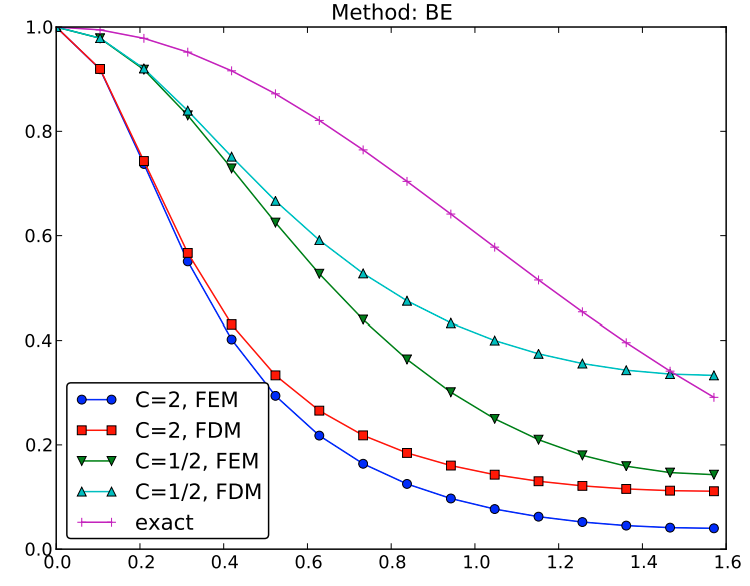
\includegraphics[width=0.7\linewidth]{img_50}
			\caption{Comparison of coarse-mesh amplification factors for Backward Euler discretization of a 1D diffusion-equation.}
			\label{fig:img_48}
		\end{figure}
	
		\begin{figure}
			\centering
			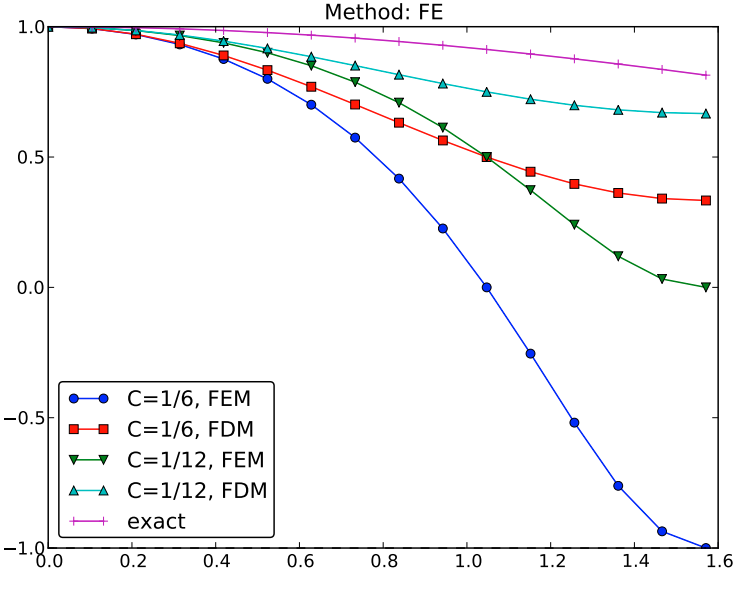
\includegraphics[width=0.7\linewidth]{img_51}
			\caption{Comparison of fine-mesh amplification factors for Forward Euler discretization of a 1D diffusion equation.}
			\label{fig:img_49}
		\end{figure}
	
		\begin{figure}
			\centering
			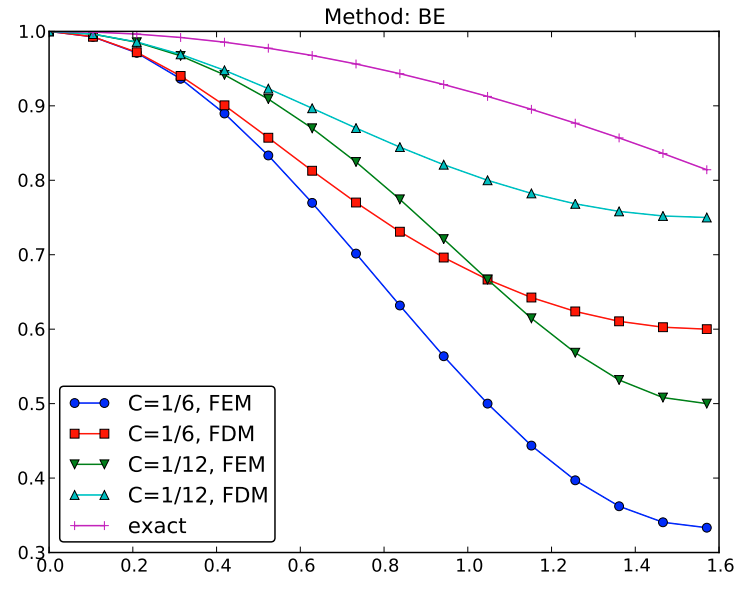
\includegraphics[width=0.7\linewidth]{img_52}
			\caption{Comparison of fine-mesh amplification factors for Backward Euler discretization of a 1D diffusion equation.}
			\label{fig:img_50}
		\end{figure}

\clearpage
\end{document} 
